
\documentclass[border=10pt, 12pt]{standalone}
\usepackage[svgnames]{xcolor}
\usepackage{amsmath}
\usepackage{pgfplots}
\pgfplotsset{compat=newest}
\usepackage[sfdefault]{FiraSans}
\usepackage{FiraMono}
\renewcommand*\familydefault{\sfdefault}
\begin{document}
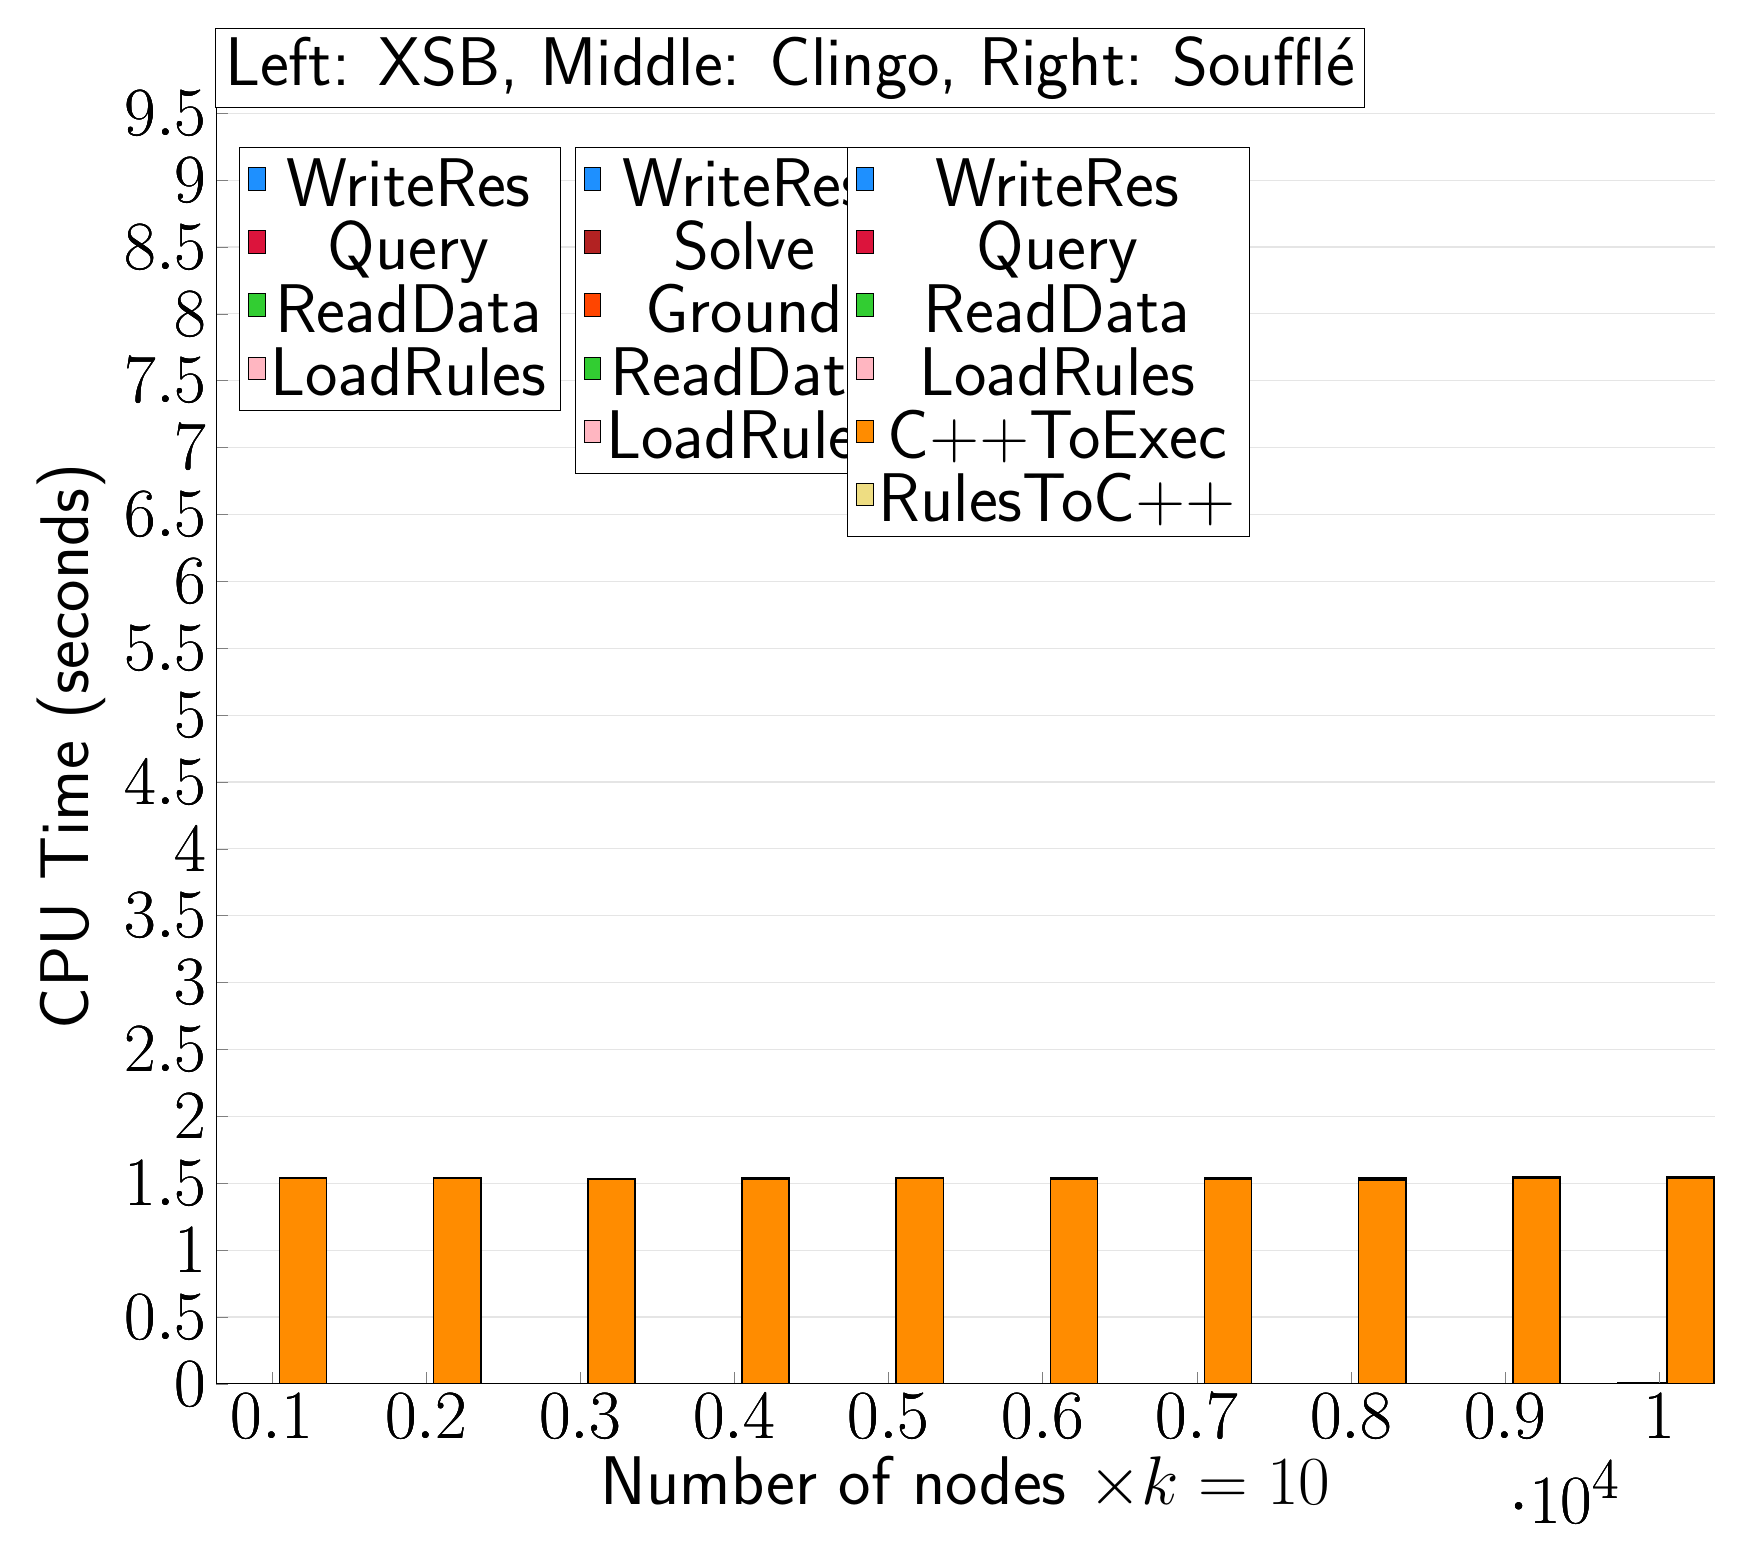
\begin{tikzpicture}
                        \begin{axis}[bar shift=-24.3pt, 
   ybar stacked,
   width=1.7\textwidth,
   bar width=0.6cm,
   ymajorgrids, tick align=inside,
   major grid style={draw=gray!20},
   xtick=data,
   ymin=0, ymax=9.536,
   axis x line*=bottom,
   axis y line*=left,
   enlarge x limits=0.04,
   legend style={
       at={(0.23, 0.97)},
       anchor=north east,
       legend columns=1,
       font=\Huge,
   },
   ylabel={CPU Time (seconds)},
   xlabel={Number of nodes $\times k=10$},
   label style={font=\Huge},
   tick label style={font=\Huge},
]
\addlegendimage{fill=DodgerBlue, draw=black, line width=0.2pt}
\addlegendentry{WriteRes}
\addlegendimage{fill=Crimson, draw=black, line width=0.2pt}
\addlegendentry{Query}
\addlegendimage{fill=LimeGreen, draw=black, line width=0.2pt}
\addlegendentry{ReadData}
\addlegendimage{fill=LightPink, draw=black, line width=0.2pt}
\addlegendentry{LoadRules}
\addplot +[fill=LightPink, draw=black, line width=0.55pt] coordinates {
(1000, 0.0005621999999999998)
(2000, 0.0005520000000000002)
(3000, 0.0005524000000000002)
(4000, 0.0005507999999999998)
(5000, 0.0005570000000000004)
(6000, 0.0005503999999999998)
(7000, 0.0005508000000000008)
(8000, 0.0005527999999999997)
(9000, 0.0005556000000000001)
(10000, 0.0005479999999999997)
};
\addplot +[fill=LimeGreen, draw=black, line width=0.55pt] coordinates {
(1000, 0.00021439999999999995)
(2000, 0.0002903999999999996)
(3000, 0.0003655999999999994)
(4000, 0.00044860000000000006)
(5000, 0.0005269999999999995)
(6000, 0.0005998000000000007)
(7000, 0.0006909999999999996)
(8000, 0.0007654000000000003)
(9000, 0.0008367999999999998)
(10000, 0.0009292000000000001)
};
\addplot +[fill=Crimson, draw=black, line width=0.55pt] coordinates {
(1000, 9.399999999999697e-06)
(2000, 9.799999999999737e-06)
(3000, 9.600000000000228e-06)
(4000, 9.400000000000029e-06)
(5000, 9.599999999999886e-06)
(6000, 1.0199999999999462e-05)
(7000, 9.99999999999994e-06)
(8000, 9.999999999999931e-06)
(9000, 1.0000000000000617e-05)
(10000, 9.399999999999686e-06)
};
\addplot +[fill=DodgerBlue, draw=black, line width=0.55pt] coordinates {
(1000, 6.40000000000005e-05)
(2000, 6.320000000000037e-05)
(3000, 6.379999999999961e-05)
(4000, 6.619999999999993e-05)
(5000, 6.33999999999999e-05)
(6000, 6.660000000000102e-05)
(7000, 6.419999999999968e-05)
(8000, 6.420000000000034e-05)
(9000, 6.699999999999969e-05)
(10000, 6.460000000000073e-05)
};
\end{axis}

\begin{axis}[bar shift=-6.5pt, 
   ybar stacked,
   width=1.7\textwidth,
   bar width=0.6cm,
   ymajorgrids, tick align=inside,
   major grid style={draw=none},
   xtick=data,
   ymin=0, ymax=9.536,
   axis x line*=none,
   axis y line*=none,
   enlarge x limits=0.04,
   legend style={
       at={(0.454, 0.97)},
       anchor=north east,
       legend columns=1,
       font=\Huge,
   },
   label style={font=\Huge},
   tick label style={font=\Huge},
]
\addlegendimage{fill=DodgerBlue, draw=black, line width=0.2pt}
\addlegendentry{WriteRes}
\addlegendimage{fill=FireBrick, draw=black, line width=0.2pt}
\addlegendentry{Solve}
\addlegendimage{fill=OrangeRed, draw=black, line width=0.2pt}
\addlegendentry{Ground}
\addlegendimage{fill=LimeGreen, draw=black, line width=0.2pt}
\addlegendentry{ReadData}
\addlegendimage{fill=LightPink, draw=black, line width=0.2pt}
\addlegendentry{LoadRules}
\addplot +[fill=LightPink, draw=black, line width=0.55pt] coordinates {
(1000, 0.0)
(2000, 0.0)
(3000, 0.0)
(4000, 0.0)
(5000, 0.0)
(6000, 0.0)
(7000, 0.0)
(8000, 0.0)
(9000, 0.0)
(10000, 0.0)
};
\addplot +[fill=LimeGreen, draw=black, line width=0.55pt] coordinates {
(1000, 0.0)
(2000, 0.0)
(3000, 0.0)
(4000, 0.0)
(5000, 0.0)
(6000, 0.0)
(7000, 0.0)
(8000, 0.0)
(9000, 0.0)
(10000, 0.0)
};
\addplot +[fill=OrangeRed, draw=black, line width=0.55pt] coordinates {
(1000, 0.0)
(2000, 0.0)
(3000, 0.0)
(4000, 0.0)
(5000, 0.0)
(6000, 0.0)
(7000, 0.0)
(8000, 0.0020000000000000018)
(9000, 0.0)
(10000, 0.0040000000000000036)
};
\addplot +[fill=FireBrick, draw=black, line width=0.55pt] coordinates {
(1000, 0.0)
(2000, 0.0)
(3000, 0.0)
(4000, 0.0)
(5000, 0.0)
(6000, 0.0)
(7000, 0.0)
(8000, 0.0)
(9000, 0.0020000000000000018)
(10000, 0.0020000000000000018)
};
\addplot +[fill=DodgerBlue, draw=black, line width=0.55pt] coordinates {
(1000, 0.0)
(2000, 0.0)
(3000, 0.0)
(4000, 0.0)
(5000, 0.0)
(6000, 0.0)
(7000, 0.0)
(8000, 0.0)
(9000, -0.0020000000000000018)
(10000, 0.0)
};
\end{axis}

\begin{axis}[bar shift=11.3pt, 
   ybar stacked,
   width=1.7\textwidth,
   bar width=0.6cm,
   ymajorgrids, tick align=inside,
   major grid style={draw=none},
   xtick=data,
   ymin=0, ymax=9.536,
   axis x line*=none,
   axis y line*=none,
   enlarge x limits=0.04,
   legend style={
       at={(0.69, 0.97)},
       anchor=north east,
       legend columns=1,
       font=\Huge,
   },
   label style={font=\Huge},
   tick label style={font=\Huge},
]
\addlegendimage{fill=DodgerBlue, draw=black, line width=0.2pt}
\addlegendentry{WriteRes}
\addlegendimage{fill=Crimson, draw=black, line width=0.2pt}
\addlegendentry{Query}
\addlegendimage{fill=LimeGreen, draw=black, line width=0.2pt}
\addlegendentry{ReadData}
\addlegendimage{fill=LightPink, draw=black, line width=0.2pt}
\addlegendentry{LoadRules}
\addlegendimage{fill=DarkOrange, draw=black, line width=0.2pt}
\addlegendentry{C++ToExec}
\addlegendimage{fill=LightGoldenrod, draw=black, line width=0.2pt}
\addlegendentry{RulesToC++}
\addplot +[fill=LightGoldenrod, draw=black, line width=0.55pt] coordinates {
(1000, 0.0020000000000000005)
(2000, 0.0020000000000000005)
(3000, 0.0)
(4000, 0.0)
(5000, 0.0)
(6000, 0.0020000000000000005)
(7000, 0.0020000000000000005)
(8000, 0.0)
(9000, 0.004000000000000002)
(10000, 0.0)
};
\addplot +[fill=DarkOrange, draw=black, line width=0.55pt] coordinates {
(1000, 1.532)
(2000, 1.5340000000000003)
(3000, 1.5299999999999998)
(4000, 1.532)
(5000, 1.534)
(6000, 1.53)
(7000, 1.528)
(8000, 1.526)
(9000, 1.53)
(10000, 1.534)
};
\addplot +[fill=LightPink, draw=black, line width=0.55pt] coordinates {
(1000, 0.0001506)
(2000, 0.0001232)
(3000, 0.00014160000000000003)
(4000, 0.0001398)
(5000, 0.0001372)
(6000, 0.00011820000000000001)
(7000, 0.00013340000000000002)
(8000, 0.00014460000000000002)
(9000, 0.0001362)
(10000, 0.0001446)
};
\addplot +[fill=LimeGreen, draw=black, line width=0.55pt] coordinates {
(1000, 0.0009258000000000001)
(2000, 0.0010802)
(3000, 0.0016348)
(4000, 0.0020311999999999995)
(5000, 0.0024955999999999997)
(6000, 0.00262)
(7000, 0.0028453999999999997)
(8000, 0.0035387999999999995)
(9000, 0.0034384)
(10000, 0.0043332)
};
\addplot +[fill=Crimson, draw=black, line width=0.55pt] coordinates {
(1000, 0.0017694000000000002)
(2000, 0.0026306)
(3000, 0.004667800000000001)
(4000, 0.005967600000000001)
(5000, 0.0065044000000000005)
(6000, 0.0077566)
(7000, 0.0089348)
(8000, 0.0102312)
(9000, 0.0108404)
(10000, 0.0124362)
};
\addplot +[fill=DodgerBlue, draw=black, line width=0.55pt] coordinates {
(1000, 0.00041720000000000006)
(2000, 0.0003038)
(3000, 0.00036339999999999994)
(4000, 0.00032399999999999996)
(5000, 0.0002784)
(6000, 0.0002562)
(7000, 0.0002578)
(8000, 0.0002944)
(9000, 0.00026940000000000004)
(10000, 0.0002792)
};
\end{axis}


\node[anchor=south, draw, fill=white] at (rel axis cs:0.42,1) {\Huge Left: XSB, Middle: Clingo, Right: Soufflé};
\end{tikzpicture}
\end{document}
                    